\documentclass[a4paper, 10pt, oneside]{report}
\usepackage{graphicx}
\graphicspath{ {images/} }


\usepackage[textwidth = 200mm,margin = 15mm]{geometry}

\usepackage{tabularx}
\setcounter{secnumdepth}{3}


\title{COS301: Application and Functional Requirements}
\date{2015-02-19}
\author{Group 3B}


\begin{document}

\maketitle
\pagenumbering{gobble}

\newpage
\pagenumbering{roman}
\tableofcontents 

\newpage
\pagenumbering{arabic}


\chapter{Introduction}

This document contains the architecture and functional requirements for the Buzz Discussion Board system. It will start with a brief  vision and background to explain the need for such a system from where the architecture and functional requirements will follow.

\chapter{Vision}

\textit{"A short discussion of the project vision, i.e. what the client is trying to achieve with the project
and the typical usage scenarios for the outputs of the project."}

\chapter{Background}

\textit "A general discussion of what lead to the project including potentially:"

\begin{itemize}
\item \textit business/research opportunities,
\item \textit opportunities to simplify/improve some aspect of life/work or community,
\item \textit problems your client is currently facing,
\item \textit ...
\end{itemize}

\chapter{Architecture requirements}

	\section{Access channel requirements}
	\section{Quality requirements}
	\section{Integration requirements}
	\section{Architecture constraints}

\chapter{ Functional requirements and application design}
	\section{Use case prioritization}
		\subsection{Critical}
		\subsection{Important}
		\subsection{Nice to have}
	\section{Use case/Services contracts}

\newpage
\documentclass[10pt]{article}
\usepackage{graphicx}
\graphicspath{ {images/} }


\usepackage[textwidth = 200mm,margin = 15mm]{geometry}

\usepackage{tabularx}

\begin{document}

\section{Use case: Groups}
	\subsection{Use case diagram}
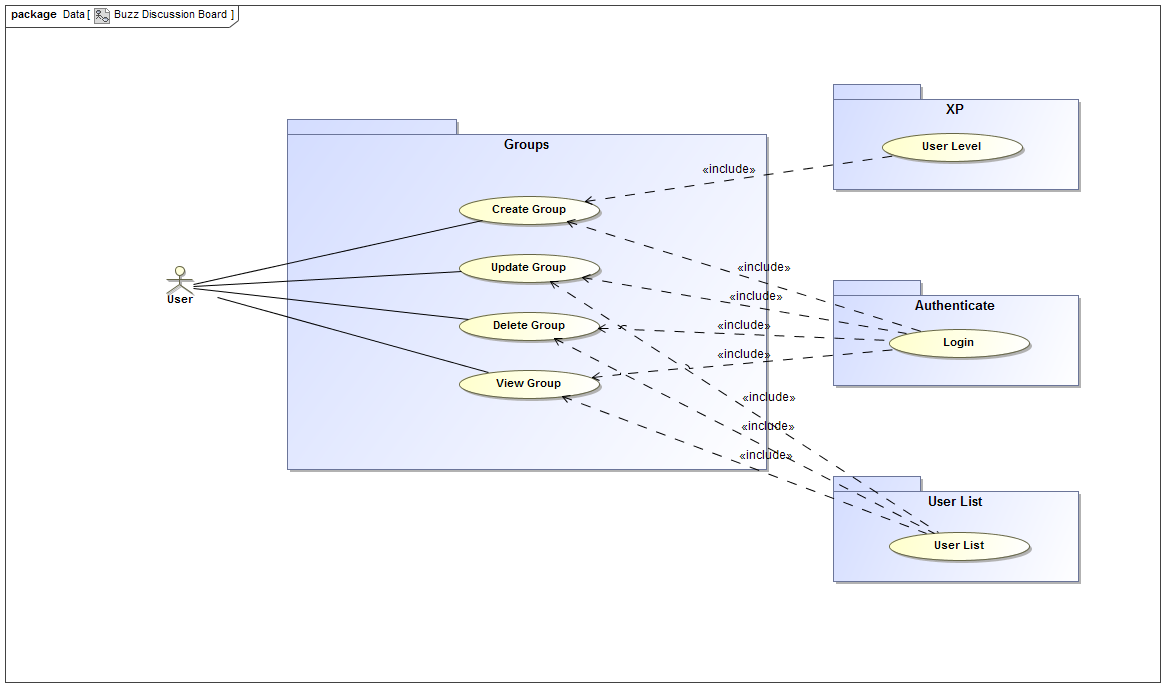
\includegraphics[width=\textwidth]{groups}
	\subsection{Short description}
	\begin{description}
		\item When a user want to create/enter a Buzz Space, first he creates a group or are part of the user-list for the group that owns the buzz space he tries to access. 
	\end{description}
	\subsection{Use cases}

\newpage
\begin{table}
\begin{tabularx}{\textwidth}{|>{\setlength\hsize{0.7\hsize}\setlength\linewidth{\hsize}}X|>{\setlength\hsize{.8\hsize}\setlength\linewidth{\hsize}}X|>{\setlength\hsize{.8\hsize}\setlength\linewidth{\hsize}}X|>{\setlength\hsize{0.7\hsize}\setlength\linewidth{\hsize}}X|}
\hline
	\multicolumn{4}{|c|}{\textbf{Use cases for Groups}}\\
\hline
	\paragraph{Use Case} & \paragraph{Preconditions} & \paragraph{Post-conditions} & \paragraph{Description} \\
\hline
	\paragraph{Create Group - User (Standard)}
&
\begin{itemize}
	\item User is logged in
	\item The group should not exist
	\item Is on XP where group creation is allowed 
\end{itemize} &
\begin{itemize}
	\item Group is created
	\item Group is saved in database
\end{itemize} &
	\paragraph{A logged in user try to create a group. Permission to create a group is dependent on the user's XP} 
	
\\
\hline
	\paragraph{Update Group}
&
\begin{itemize}
	\item User is logged in
	\item The group should exist
	\item Is part of the user-list for that group
	\item Is set to admin for the group in the user-list
\end{itemize} &
\begin{itemize}
	\item Group details is changed
	\item Changes are saved in database
	\item All members of group is notified
\end{itemize} &
	\paragraph{Changes to the group's details can only be made by the admins of the group as set out in the user-list}
\\

\hline

	\paragraph{Delete Group}
&
\begin{itemize}
	\item User is logged in
	\item The group should exist
	\item Is part of the user-list for that group
	\item Is set to admin for the group in the user-list
\end{itemize} &
\begin{itemize}
	\item Group is deleted
	\item Group is marked as deleted in database
	\item All members of group is notified
\end{itemize} &
	\paragraph{Deleting a group can only be done by the admins of the group as set out in the user-list}
\\
\hline

	\paragraph{View Group}
&
\begin{itemize}
	\item The group should exist
	\item The group should be publicly visible	
\end{itemize} &
\begin{itemize}
	\item Group details are accessed
\end{itemize} &
	\paragraph{Anyone can view the group's info if the group is a public group}
\\
\hline
	\paragraph{View Group - Hidden}
&
\begin{itemize}
	\item User is logged in
	\item The group should exist
	\item Is part of the user-list for that group
\end{itemize} &
\begin{itemize}
	\item Group details are accessed
\end{itemize} &
	\paragraph{Anyone in the group's user-list can view the group's info when the group is a hidden group}
\\
\hline


\end{tabularx}
\end{table}

\newpage
\begin{table}
\begin{tabularx}{\textwidth}{|>{\setlength\hsize{0.7\hsize}\setlength\linewidth{\hsize}}X|>{\setlength\hsize{.8\hsize}\setlength\linewidth{\hsize}}X|>{\setlength\hsize{.8\hsize}\setlength\linewidth{\hsize}}X|>{\setlength\hsize{0.7\hsize}\setlength\linewidth{\hsize}}X|}
\hline
	\multicolumn{4}{|c|}{\textbf{Use cases for Groups}}\\
\hline
	\paragraph{Use Case} & \paragraph{Preconditions} & \paragraph{Post-conditions} & \paragraph{Description} \\
	\paragraph{Create Group - User (Admin)}
&
\begin{itemize}
	\item User is logged in as Admin
	\item The group should not exist
\end{itemize} &
\begin{itemize}
	\item Group is created
	\item Group is saved in database
\end{itemize} &
	\paragraph{A logged in Admin can add a group. } 
	
\\
\hline
	\paragraph{Update Group - Admin}
&
\begin{itemize}
	\item User is logged in as Admin
	\item The group should exist
\end{itemize} &
\begin{itemize}
	\item Group details is changed
	\item Changes are saved in database
	\item All members of group is notified
\end{itemize} &
	\paragraph{Changes to the group's details can only be made by the admins of the buzz system}
\\

\hline

	\paragraph{Delete Group - Admin}
&
\begin{itemize}
	\item User is logged in as Admin
	\item The group should exist
\end{itemize} &
\begin{itemize}
	\item Group is deleted
	\item Group is marked as deleted in database
	\item All members of group is notified
\end{itemize} &
	\paragraph{Deleting a group can be done by the admins of the buzz system}
\\
\hline





\end{tabularx}
\end{table}


\end{document}
\newpage
	\section{Use case: Spaces}
	\subsection{Use case diagram}
	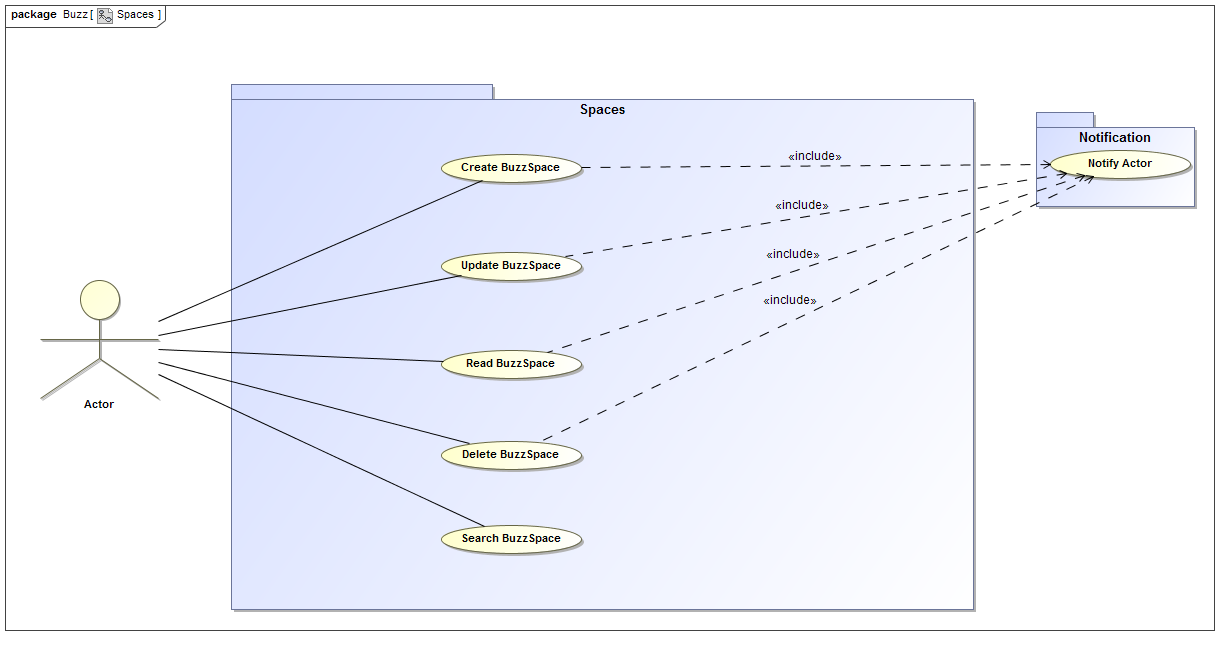
\includegraphics[width=\textwidth]{spacesUseCase}
	\subsection{Short description}
	\begin{description}
		
		\item[] 
			The following section will discuss the functional requirements of the Spaces section of the BuzzSpace program.
		
		\item[] Different actors:
		\begin{itemize}
			\item Administrator: Has system wide permission.
			\item Lecturer: Has full permission for the current BuzzSpace
			\item User: Has permission for the current BuzzSpace according to the users XP. Lecturer will included in users as they will be assigned the required XP.   
		\end{itemize}
		
	\end{description}
	
	\subsection{Use case prioritization}
	\begin{description}
		\item[] Critical
		\begin{itemize}
			\item Create BuzzSpace
			\item Delete BuzzSpace
			\item Update BuzzSpace
			\item Read BuzzSpace
			\item Authentication
		\end{itemize}
		
		\item[] Important
		\begin{itemize}
			\item Search BuzzSpaces
			\item Check XP
		\end{itemize}
	\end{description}
	
	\subsection{Use cases}
	\newpage
	\begin{longtable}{@{}|p{1.5cm}|p{2.2cm}|p{3cm}|p{3.5cm}|p{3.5cm}|@{}}
		\toprule
		\multicolumn{5}{|c|}{\textbf{Use cases for Space}}\\
		\hline
		\textbf{Actor} & \textbf{Use Case} & \textbf{Pre-condition} & \textbf{Post-Conditions} & \textbf{Description} \\ \midrule
		
		User Or Admin& 
		Create BuzzSpace& 
		\begin{itemize}
			\item A group must exist
			\item The actor has permission
			\item The actor has the required amount of XP
		\end{itemize}& 
		\begin{itemize}
			\item Space created
		\end{itemize} & 
		Create a new BuzzSpace (discussion space within group) \\ \midrule
		
		User Or Admin& 
		Delete BuzzSpace& 
		\begin{itemize}
			\item The BuzzSpace exists that wants to be removed
			\item The actor has permission
			\item The actor has the required amount of XP
		\end{itemize}& 
		\begin{itemize}
			\item BuzzSpace removed from groups
		\end{itemize} & 
		Remove a BuzzSpace from groups and notify the users belonging to that group \\ \midrule
		
		User Or Admin& 
		Update BuzzSpace& 
		\begin{itemize}
			\item The Space exists that needs to be updated
			\item The actor has permission
			\item The actor has the required amount of XP
		\end{itemize}& 
		\begin{itemize}
			\item State of space changed
		\end{itemize} & 
		Allow users with permission to update the BuzzSpace \\ \midrule
		
		User Or Admin& 
		Read BuzzSpace& 
		\begin{itemize}
			\item The Space exists
			\item The actor has permission
		\end{itemize}& 
		\begin{itemize}
			\item BuzzSpace marked read
		\end{itemize} & 
		Allow users with permission to read the BuzzSpaces \\ \midrule
		
		User Or Admin& 
		Search BuzzSpaces& 
		\begin{itemize}
			\item Must be a registered user
		\end{itemize}& 
		\begin{itemize}
			\item Search list created
		\end{itemize} & 
		Search the BuzzSpaces in groups \\ \midrule
		
		User Or Admin& 
		Authentication& 
		\begin{itemize}
			\item Actor must be registered
			\item Actor must be logged into the Buzz System 
		\end{itemize}& 
		\begin{itemize}
			\item Actor grated access
		\end{itemize} & 
		See if the Actor is authenticated to the system \\ \midrule
		
		User Or Admin& 
		Check XP& 
		\begin{itemize}
			\item Actor must be registered
			\item Actor must be logged into the Buzz System 
			\item Actor has the required amount of XP
		\end{itemize}& 
		\begin{itemize}
			\item Actor allowed to make changes
		\end{itemize} & 
		See if the Actor has the required amount of XP to be allowed to make changes to the BuzzSpace \\ \bottomrule
		
	\end{longtable}
\newpage
\documentclass[10pt]{article}
\usepackage{graphicx}
\graphicspath{ {images/} }


\usepackage[textwidth = 200mm,margin = 15mm]{geometry}

\usepackage{tabularx}

\begin{document}

\section{Use case: Groups}
	\subsection{Use case diagram}
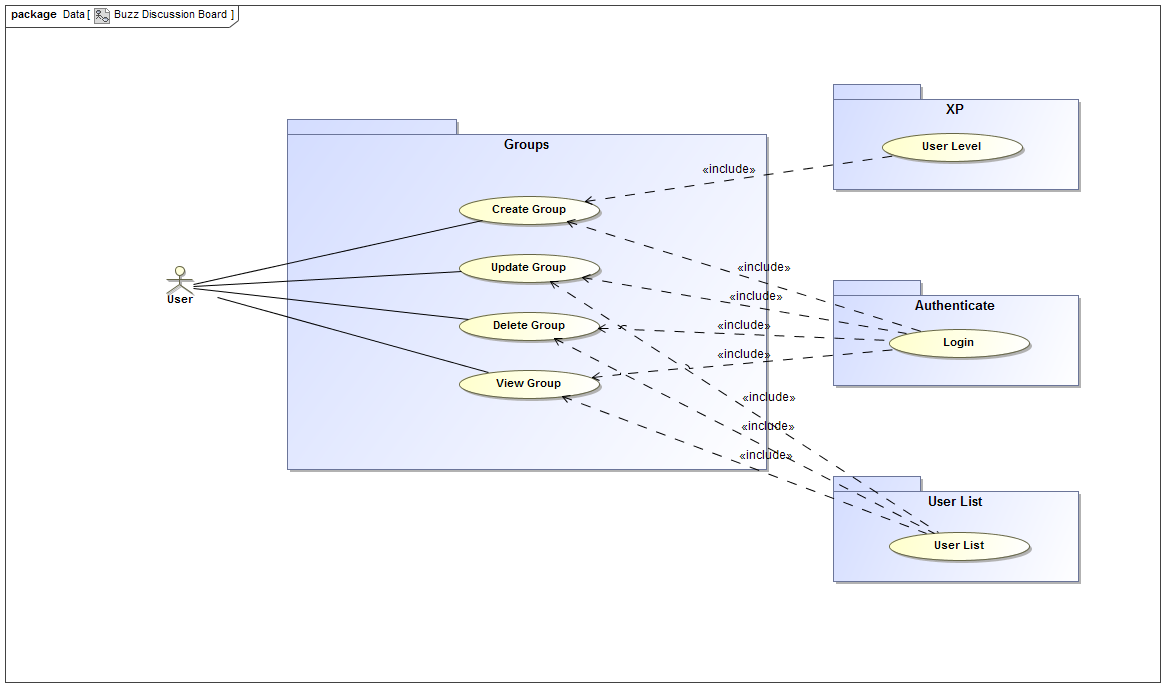
\includegraphics[width=\textwidth]{groups}
	\subsection{Short description}
	\begin{description}
		\item When a user want to create/enter a Buzz Space, first he creates a group or are part of the user-list for the group that owns the buzz space he tries to access. 
	\end{description}
	\subsection{Use cases}

\newpage
\begin{table}
\begin{tabularx}{\textwidth}{|>{\setlength\hsize{0.7\hsize}\setlength\linewidth{\hsize}}X|>{\setlength\hsize{.8\hsize}\setlength\linewidth{\hsize}}X|>{\setlength\hsize{.8\hsize}\setlength\linewidth{\hsize}}X|>{\setlength\hsize{0.7\hsize}\setlength\linewidth{\hsize}}X|}
\hline
	\multicolumn{4}{|c|}{\textbf{Use cases for Groups}}\\
\hline
	\paragraph{Use Case} & \paragraph{Preconditions} & \paragraph{Post-conditions} & \paragraph{Description} \\
\hline
	\paragraph{Create Group - User (Standard)}
&
\begin{itemize}
	\item User is logged in
	\item The group should not exist
	\item Is on XP where group creation is allowed 
\end{itemize} &
\begin{itemize}
	\item Group is created
	\item Group is saved in database
\end{itemize} &
	\paragraph{A logged in user try to create a group. Permission to create a group is dependent on the user's XP} 
	
\\
\hline
	\paragraph{Update Group}
&
\begin{itemize}
	\item User is logged in
	\item The group should exist
	\item Is part of the user-list for that group
	\item Is set to admin for the group in the user-list
\end{itemize} &
\begin{itemize}
	\item Group details is changed
	\item Changes are saved in database
	\item All members of group is notified
\end{itemize} &
	\paragraph{Changes to the group's details can only be made by the admins of the group as set out in the user-list}
\\

\hline

	\paragraph{Delete Group}
&
\begin{itemize}
	\item User is logged in
	\item The group should exist
	\item Is part of the user-list for that group
	\item Is set to admin for the group in the user-list
\end{itemize} &
\begin{itemize}
	\item Group is deleted
	\item Group is marked as deleted in database
	\item All members of group is notified
\end{itemize} &
	\paragraph{Deleting a group can only be done by the admins of the group as set out in the user-list}
\\
\hline

	\paragraph{View Group}
&
\begin{itemize}
	\item The group should exist
	\item The group should be publicly visible	
\end{itemize} &
\begin{itemize}
	\item Group details are accessed
\end{itemize} &
	\paragraph{Anyone can view the group's info if the group is a public group}
\\
\hline
	\paragraph{View Group - Hidden}
&
\begin{itemize}
	\item User is logged in
	\item The group should exist
	\item Is part of the user-list for that group
\end{itemize} &
\begin{itemize}
	\item Group details are accessed
\end{itemize} &
	\paragraph{Anyone in the group's user-list can view the group's info when the group is a hidden group}
\\
\hline


\end{tabularx}
\end{table}

\newpage
\begin{table}
\begin{tabularx}{\textwidth}{|>{\setlength\hsize{0.7\hsize}\setlength\linewidth{\hsize}}X|>{\setlength\hsize{.8\hsize}\setlength\linewidth{\hsize}}X|>{\setlength\hsize{.8\hsize}\setlength\linewidth{\hsize}}X|>{\setlength\hsize{0.7\hsize}\setlength\linewidth{\hsize}}X|}
\hline
	\multicolumn{4}{|c|}{\textbf{Use cases for Groups}}\\
\hline
	\paragraph{Use Case} & \paragraph{Preconditions} & \paragraph{Post-conditions} & \paragraph{Description} \\
	\paragraph{Create Group - User (Admin)}
&
\begin{itemize}
	\item User is logged in as Admin
	\item The group should not exist
\end{itemize} &
\begin{itemize}
	\item Group is created
	\item Group is saved in database
\end{itemize} &
	\paragraph{A logged in Admin can add a group. } 
	
\\
\hline
	\paragraph{Update Group - Admin}
&
\begin{itemize}
	\item User is logged in as Admin
	\item The group should exist
\end{itemize} &
\begin{itemize}
	\item Group details is changed
	\item Changes are saved in database
	\item All members of group is notified
\end{itemize} &
	\paragraph{Changes to the group's details can only be made by the admins of the buzz system}
\\

\hline

	\paragraph{Delete Group - Admin}
&
\begin{itemize}
	\item User is logged in as Admin
	\item The group should exist
\end{itemize} &
\begin{itemize}
	\item Group is deleted
	\item Group is marked as deleted in database
	\item All members of group is notified
\end{itemize} &
	\paragraph{Deleting a group can be done by the admins of the buzz system}
\\
\hline





\end{tabularx}
\end{table}


\end{document}
\newpage
\documentclass[10pt]{article}
\usepackage{graphicx}
\graphicspath{ {images/} }


\usepackage[textwidth = 200mm,margin = 15mm]{geometry}

\usepackage{tabularx}

\begin{document}

\section{Use case: Groups}
	\subsection{Use case diagram}
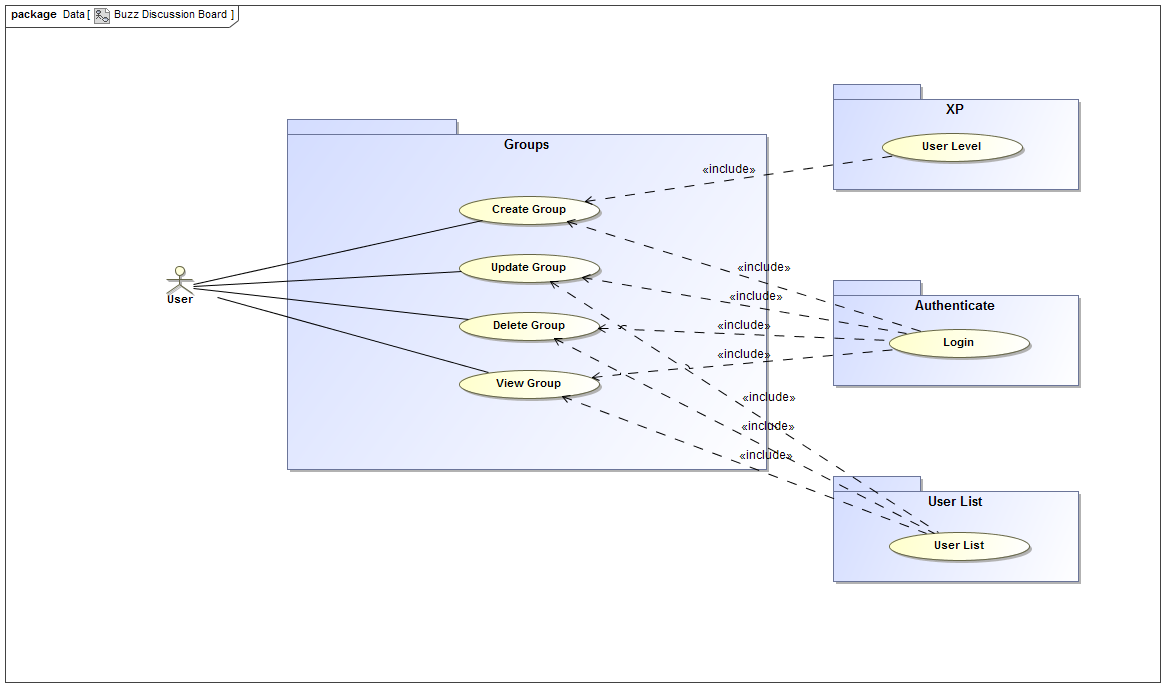
\includegraphics[width=\textwidth]{groups}
	\subsection{Short description}
	\begin{description}
		\item When a user want to create/enter a Buzz Space, first he creates a group or are part of the user-list for the group that owns the buzz space he tries to access. 
	\end{description}
	\subsection{Use cases}

\newpage
\begin{table}
\begin{tabularx}{\textwidth}{|>{\setlength\hsize{0.7\hsize}\setlength\linewidth{\hsize}}X|>{\setlength\hsize{.8\hsize}\setlength\linewidth{\hsize}}X|>{\setlength\hsize{.8\hsize}\setlength\linewidth{\hsize}}X|>{\setlength\hsize{0.7\hsize}\setlength\linewidth{\hsize}}X|}
\hline
	\multicolumn{4}{|c|}{\textbf{Use cases for Groups}}\\
\hline
	\paragraph{Use Case} & \paragraph{Preconditions} & \paragraph{Post-conditions} & \paragraph{Description} \\
\hline
	\paragraph{Create Group - User (Standard)}
&
\begin{itemize}
	\item User is logged in
	\item The group should not exist
	\item Is on XP where group creation is allowed 
\end{itemize} &
\begin{itemize}
	\item Group is created
	\item Group is saved in database
\end{itemize} &
	\paragraph{A logged in user try to create a group. Permission to create a group is dependent on the user's XP} 
	
\\
\hline
	\paragraph{Update Group}
&
\begin{itemize}
	\item User is logged in
	\item The group should exist
	\item Is part of the user-list for that group
	\item Is set to admin for the group in the user-list
\end{itemize} &
\begin{itemize}
	\item Group details is changed
	\item Changes are saved in database
	\item All members of group is notified
\end{itemize} &
	\paragraph{Changes to the group's details can only be made by the admins of the group as set out in the user-list}
\\

\hline

	\paragraph{Delete Group}
&
\begin{itemize}
	\item User is logged in
	\item The group should exist
	\item Is part of the user-list for that group
	\item Is set to admin for the group in the user-list
\end{itemize} &
\begin{itemize}
	\item Group is deleted
	\item Group is marked as deleted in database
	\item All members of group is notified
\end{itemize} &
	\paragraph{Deleting a group can only be done by the admins of the group as set out in the user-list}
\\
\hline

	\paragraph{View Group}
&
\begin{itemize}
	\item The group should exist
	\item The group should be publicly visible	
\end{itemize} &
\begin{itemize}
	\item Group details are accessed
\end{itemize} &
	\paragraph{Anyone can view the group's info if the group is a public group}
\\
\hline
	\paragraph{View Group - Hidden}
&
\begin{itemize}
	\item User is logged in
	\item The group should exist
	\item Is part of the user-list for that group
\end{itemize} &
\begin{itemize}
	\item Group details are accessed
\end{itemize} &
	\paragraph{Anyone in the group's user-list can view the group's info when the group is a hidden group}
\\
\hline


\end{tabularx}
\end{table}

\newpage
\begin{table}
\begin{tabularx}{\textwidth}{|>{\setlength\hsize{0.7\hsize}\setlength\linewidth{\hsize}}X|>{\setlength\hsize{.8\hsize}\setlength\linewidth{\hsize}}X|>{\setlength\hsize{.8\hsize}\setlength\linewidth{\hsize}}X|>{\setlength\hsize{0.7\hsize}\setlength\linewidth{\hsize}}X|}
\hline
	\multicolumn{4}{|c|}{\textbf{Use cases for Groups}}\\
\hline
	\paragraph{Use Case} & \paragraph{Preconditions} & \paragraph{Post-conditions} & \paragraph{Description} \\
	\paragraph{Create Group - User (Admin)}
&
\begin{itemize}
	\item User is logged in as Admin
	\item The group should not exist
\end{itemize} &
\begin{itemize}
	\item Group is created
	\item Group is saved in database
\end{itemize} &
	\paragraph{A logged in Admin can add a group. } 
	
\\
\hline
	\paragraph{Update Group - Admin}
&
\begin{itemize}
	\item User is logged in as Admin
	\item The group should exist
\end{itemize} &
\begin{itemize}
	\item Group details is changed
	\item Changes are saved in database
	\item All members of group is notified
\end{itemize} &
	\paragraph{Changes to the group's details can only be made by the admins of the buzz system}
\\

\hline

	\paragraph{Delete Group - Admin}
&
\begin{itemize}
	\item User is logged in as Admin
	\item The group should exist
\end{itemize} &
\begin{itemize}
	\item Group is deleted
	\item Group is marked as deleted in database
	\item All members of group is notified
\end{itemize} &
	\paragraph{Deleting a group can be done by the admins of the buzz system}
\\
\hline





\end{tabularx}
\end{table}


\end{document}
\newpage
\documentclass[10pt]{article}
\usepackage{graphicx}
\graphicspath{ {images/} }


\usepackage[textwidth = 200mm,margin = 15mm]{geometry}

\usepackage{tabularx}

\begin{document}

\section{Use case: Groups}
	\subsection{Use case diagram}
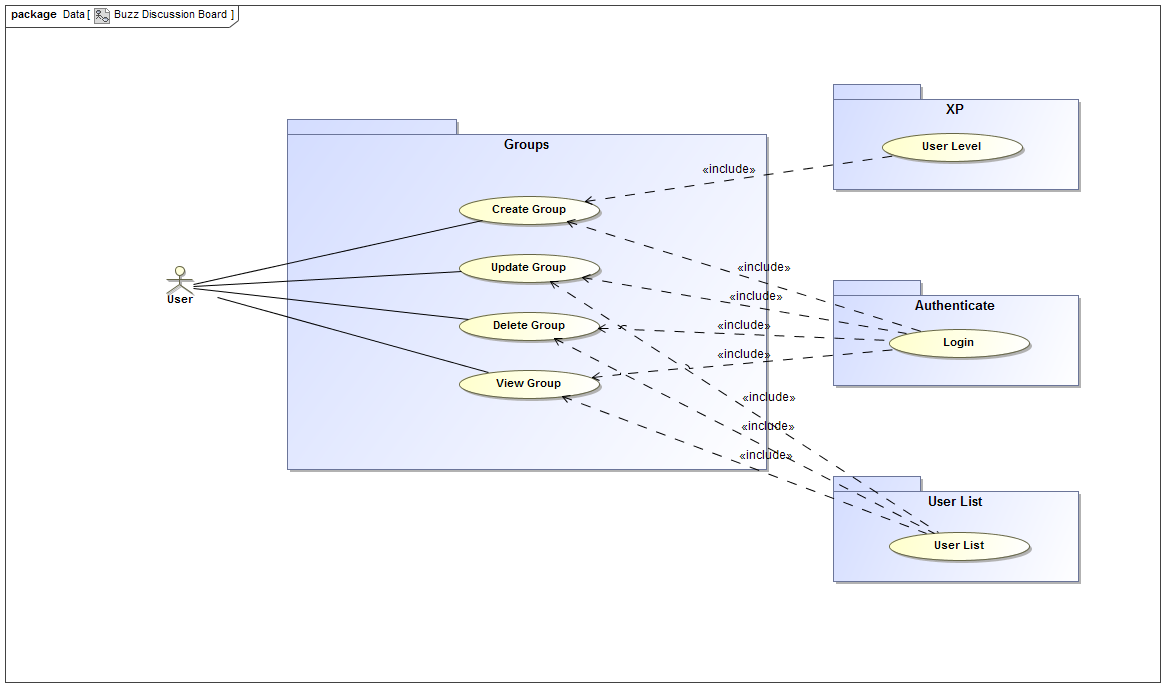
\includegraphics[width=\textwidth]{groups}
	\subsection{Short description}
	\begin{description}
		\item When a user want to create/enter a Buzz Space, first he creates a group or are part of the user-list for the group that owns the buzz space he tries to access. 
	\end{description}
	\subsection{Use cases}

\newpage
\begin{table}
\begin{tabularx}{\textwidth}{|>{\setlength\hsize{0.7\hsize}\setlength\linewidth{\hsize}}X|>{\setlength\hsize{.8\hsize}\setlength\linewidth{\hsize}}X|>{\setlength\hsize{.8\hsize}\setlength\linewidth{\hsize}}X|>{\setlength\hsize{0.7\hsize}\setlength\linewidth{\hsize}}X|}
\hline
	\multicolumn{4}{|c|}{\textbf{Use cases for Groups}}\\
\hline
	\paragraph{Use Case} & \paragraph{Preconditions} & \paragraph{Post-conditions} & \paragraph{Description} \\
\hline
	\paragraph{Create Group - User (Standard)}
&
\begin{itemize}
	\item User is logged in
	\item The group should not exist
	\item Is on XP where group creation is allowed 
\end{itemize} &
\begin{itemize}
	\item Group is created
	\item Group is saved in database
\end{itemize} &
	\paragraph{A logged in user try to create a group. Permission to create a group is dependent on the user's XP} 
	
\\
\hline
	\paragraph{Update Group}
&
\begin{itemize}
	\item User is logged in
	\item The group should exist
	\item Is part of the user-list for that group
	\item Is set to admin for the group in the user-list
\end{itemize} &
\begin{itemize}
	\item Group details is changed
	\item Changes are saved in database
	\item All members of group is notified
\end{itemize} &
	\paragraph{Changes to the group's details can only be made by the admins of the group as set out in the user-list}
\\

\hline

	\paragraph{Delete Group}
&
\begin{itemize}
	\item User is logged in
	\item The group should exist
	\item Is part of the user-list for that group
	\item Is set to admin for the group in the user-list
\end{itemize} &
\begin{itemize}
	\item Group is deleted
	\item Group is marked as deleted in database
	\item All members of group is notified
\end{itemize} &
	\paragraph{Deleting a group can only be done by the admins of the group as set out in the user-list}
\\
\hline

	\paragraph{View Group}
&
\begin{itemize}
	\item The group should exist
	\item The group should be publicly visible	
\end{itemize} &
\begin{itemize}
	\item Group details are accessed
\end{itemize} &
	\paragraph{Anyone can view the group's info if the group is a public group}
\\
\hline
	\paragraph{View Group - Hidden}
&
\begin{itemize}
	\item User is logged in
	\item The group should exist
	\item Is part of the user-list for that group
\end{itemize} &
\begin{itemize}
	\item Group details are accessed
\end{itemize} &
	\paragraph{Anyone in the group's user-list can view the group's info when the group is a hidden group}
\\
\hline


\end{tabularx}
\end{table}

\newpage
\begin{table}
\begin{tabularx}{\textwidth}{|>{\setlength\hsize{0.7\hsize}\setlength\linewidth{\hsize}}X|>{\setlength\hsize{.8\hsize}\setlength\linewidth{\hsize}}X|>{\setlength\hsize{.8\hsize}\setlength\linewidth{\hsize}}X|>{\setlength\hsize{0.7\hsize}\setlength\linewidth{\hsize}}X|}
\hline
	\multicolumn{4}{|c|}{\textbf{Use cases for Groups}}\\
\hline
	\paragraph{Use Case} & \paragraph{Preconditions} & \paragraph{Post-conditions} & \paragraph{Description} \\
	\paragraph{Create Group - User (Admin)}
&
\begin{itemize}
	\item User is logged in as Admin
	\item The group should not exist
\end{itemize} &
\begin{itemize}
	\item Group is created
	\item Group is saved in database
\end{itemize} &
	\paragraph{A logged in Admin can add a group. } 
	
\\
\hline
	\paragraph{Update Group - Admin}
&
\begin{itemize}
	\item User is logged in as Admin
	\item The group should exist
\end{itemize} &
\begin{itemize}
	\item Group details is changed
	\item Changes are saved in database
	\item All members of group is notified
\end{itemize} &
	\paragraph{Changes to the group's details can only be made by the admins of the buzz system}
\\

\hline

	\paragraph{Delete Group - Admin}
&
\begin{itemize}
	\item User is logged in as Admin
	\item The group should exist
\end{itemize} &
\begin{itemize}
	\item Group is deleted
	\item Group is marked as deleted in database
	\item All members of group is notified
\end{itemize} &
	\paragraph{Deleting a group can be done by the admins of the buzz system}
\\
\hline





\end{tabularx}
\end{table}


\end{document}
\newpage
\documentclass[10pt]{article}
\usepackage{graphicx}
\graphicspath{ {images/} }


\usepackage[textwidth = 200mm,margin = 15mm]{geometry}

\usepackage{tabularx}

\begin{document}

\section{Use case: Groups}
	\subsection{Use case diagram}
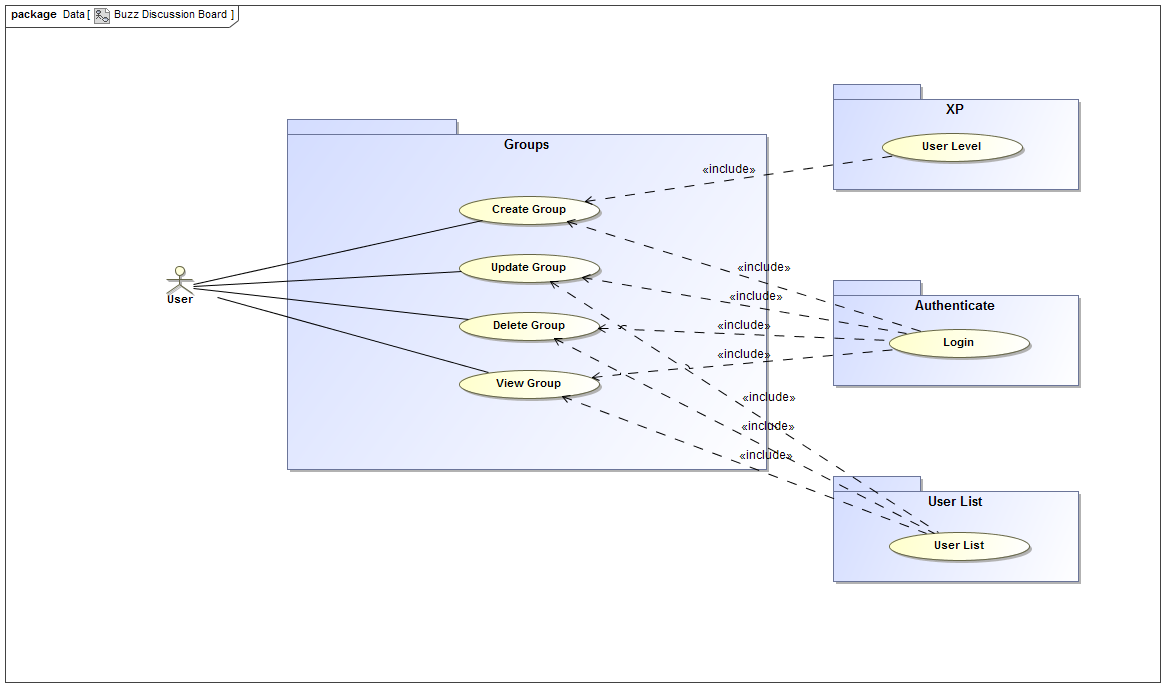
\includegraphics[width=\textwidth]{groups}
	\subsection{Short description}
	\begin{description}
		\item When a user want to create/enter a Buzz Space, first he creates a group or are part of the user-list for the group that owns the buzz space he tries to access. 
	\end{description}
	\subsection{Use cases}

\newpage
\begin{table}
\begin{tabularx}{\textwidth}{|>{\setlength\hsize{0.7\hsize}\setlength\linewidth{\hsize}}X|>{\setlength\hsize{.8\hsize}\setlength\linewidth{\hsize}}X|>{\setlength\hsize{.8\hsize}\setlength\linewidth{\hsize}}X|>{\setlength\hsize{0.7\hsize}\setlength\linewidth{\hsize}}X|}
\hline
	\multicolumn{4}{|c|}{\textbf{Use cases for Groups}}\\
\hline
	\paragraph{Use Case} & \paragraph{Preconditions} & \paragraph{Post-conditions} & \paragraph{Description} \\
\hline
	\paragraph{Create Group - User (Standard)}
&
\begin{itemize}
	\item User is logged in
	\item The group should not exist
	\item Is on XP where group creation is allowed 
\end{itemize} &
\begin{itemize}
	\item Group is created
	\item Group is saved in database
\end{itemize} &
	\paragraph{A logged in user try to create a group. Permission to create a group is dependent on the user's XP} 
	
\\
\hline
	\paragraph{Update Group}
&
\begin{itemize}
	\item User is logged in
	\item The group should exist
	\item Is part of the user-list for that group
	\item Is set to admin for the group in the user-list
\end{itemize} &
\begin{itemize}
	\item Group details is changed
	\item Changes are saved in database
	\item All members of group is notified
\end{itemize} &
	\paragraph{Changes to the group's details can only be made by the admins of the group as set out in the user-list}
\\

\hline

	\paragraph{Delete Group}
&
\begin{itemize}
	\item User is logged in
	\item The group should exist
	\item Is part of the user-list for that group
	\item Is set to admin for the group in the user-list
\end{itemize} &
\begin{itemize}
	\item Group is deleted
	\item Group is marked as deleted in database
	\item All members of group is notified
\end{itemize} &
	\paragraph{Deleting a group can only be done by the admins of the group as set out in the user-list}
\\
\hline

	\paragraph{View Group}
&
\begin{itemize}
	\item The group should exist
	\item The group should be publicly visible	
\end{itemize} &
\begin{itemize}
	\item Group details are accessed
\end{itemize} &
	\paragraph{Anyone can view the group's info if the group is a public group}
\\
\hline
	\paragraph{View Group - Hidden}
&
\begin{itemize}
	\item User is logged in
	\item The group should exist
	\item Is part of the user-list for that group
\end{itemize} &
\begin{itemize}
	\item Group details are accessed
\end{itemize} &
	\paragraph{Anyone in the group's user-list can view the group's info when the group is a hidden group}
\\
\hline


\end{tabularx}
\end{table}

\newpage
\begin{table}
\begin{tabularx}{\textwidth}{|>{\setlength\hsize{0.7\hsize}\setlength\linewidth{\hsize}}X|>{\setlength\hsize{.8\hsize}\setlength\linewidth{\hsize}}X|>{\setlength\hsize{.8\hsize}\setlength\linewidth{\hsize}}X|>{\setlength\hsize{0.7\hsize}\setlength\linewidth{\hsize}}X|}
\hline
	\multicolumn{4}{|c|}{\textbf{Use cases for Groups}}\\
\hline
	\paragraph{Use Case} & \paragraph{Preconditions} & \paragraph{Post-conditions} & \paragraph{Description} \\
	\paragraph{Create Group - User (Admin)}
&
\begin{itemize}
	\item User is logged in as Admin
	\item The group should not exist
\end{itemize} &
\begin{itemize}
	\item Group is created
	\item Group is saved in database
\end{itemize} &
	\paragraph{A logged in Admin can add a group. } 
	
\\
\hline
	\paragraph{Update Group - Admin}
&
\begin{itemize}
	\item User is logged in as Admin
	\item The group should exist
\end{itemize} &
\begin{itemize}
	\item Group details is changed
	\item Changes are saved in database
	\item All members of group is notified
\end{itemize} &
	\paragraph{Changes to the group's details can only be made by the admins of the buzz system}
\\

\hline

	\paragraph{Delete Group - Admin}
&
\begin{itemize}
	\item User is logged in as Admin
	\item The group should exist
\end{itemize} &
\begin{itemize}
	\item Group is deleted
	\item Group is marked as deleted in database
	\item All members of group is notified
\end{itemize} &
	\paragraph{Deleting a group can be done by the admins of the buzz system}
\\
\hline





\end{tabularx}
\end{table}


\end{document}
\newpage

\subsection{Required functionality}
\subsection{Process specifications}
\subsection{Domain Model}
\subsection{Open Issues}



\end{document}

